\documentclass[conference]{IEEEtran}

\usepackage{graphicx}
\usepackage{amsmath}
\usepackage{booktabs}
\usepackage{url}

\title{
	Deep Learning-Based Crater Detection Using YOLOv8,
	Faster R-CNN, and RetinaNet
}

\author{
	\IEEEauthorblockN{Scott Nguyen}
	\IEEEauthorblockA{
		Department of Electrical and Computer Engineering \\
		University of New Mexico \\
		Albuquerque, New Mexico, USA \\
		snguyen9@unm.edu
	}
}

\begin{document}
	
	\maketitle
	
	\begin{abstract}
		
		Crater detection remains an important problem for autonomous planetary exploration because surface hazards such as craters and rough terrain can negatively affect rover navigation and landing operations. This project investigates deep learning-based object detection methods for planetary crater detection using bounding-box annotations on planetary surface imagery. A complete end-to-end crater detection pipeline was developed, including dataset verification, ground-truth visualization, model training, prediction generation, and comparative evaluation. Three deep learning object detection models were implemented and evaluated: YOLOv8, Faster R-CNN, and RetinaNet. The dataset was organized into training, validation, and testing splits using YOLO-format bounding-box labels. Ground-truth annotations were visualized and verified prior to training to ensure dataset integrity. Experimental results demonstrated that YOLOv8 achieved the best overall performance, obtaining an mAP@0.5 of approximately 0.70 on the test dataset, while Faster R-CNN achieved comparable performance with slightly lower accuracy. RetinaNet underperformed under limited training conditions and dataset size constraints. Comparative analysis shows that one-stage detectors such as YOLOv8 can provide strong crater detection performance while maintaining computational efficiency. The developed framework demonstrates the feasibility of applying modern deep learning object detection techniques to planetary crater detection tasks and provides a foundation for future work involving larger datasets, GPU acceleration, and foundation-model-based approaches.
		
	\end{abstract}
	
	\begin{IEEEkeywords}
		planetary exploration, crater detection, deep learning, object detection, YOLOv8, Faster R-CNN, RetinaNet, computer vision
	\end{IEEEkeywords}
	
	\section{Introduction}
	
	Planetary exploration continues to be an important area of research for both scientific discovery and the development of future autonomous space missions. The Moon and Mars remain major targets for robotic exploration because they provide opportunities for scientific analysis, infrastructure development, and long-term planetary operations. However, planetary surfaces contain numerous hazards including craters, rocks, steep terrain, and rough surface features that can negatively affect autonomous rover navigation, landing systems, and mission safety.
	
	Crater detection is therefore an important computer vision problem for autonomous planetary exploration systems. Accurate crater detection can support hazard avoidance, terrain mapping, localization, navigation, and autonomous landing operations. Traditional crater detection methods often rely on handcrafted image processing techniques such as edge detection, thresholding, or Hough-transform-based approaches. Although these methods can detect some crater structures, they may struggle under varying illumination conditions, low contrast, overlapping terrain features, or noisy planetary imagery.
	
	Recent advances in deep learning and computer vision have significantly improved object detection performance across many domains. Deep learning-based object detection methods are capable of automatically learning complex spatial and visual features directly from image data. Modern object detection architectures such as YOLO, Faster R-CNN, and RetinaNet have demonstrated strong performance in applications including autonomous driving, aerial imaging, medical imaging, and robotic perception. These approaches provide an opportunity to improve crater detection performance on planetary imagery while reducing the need for manually engineered feature extraction methods.
	
	Previous work in planetary image analysis has also explored semantic segmentation approaches such as U-Net for terrain and rock segmentation. While segmentation methods provide pixel-level classification, object detection methods offer advantages for identifying crater locations using compact bounding-box representations. Bounding-box-based crater detection can reduce annotation complexity while enabling efficient object localization and evaluation using standard object detection metrics.
	
	This project investigates deep learning-based crater detection using bounding-box object detection methods on planetary surface imagery. A complete end-to-end crater detection pipeline was developed, including dataset verification, ground-truth visualization, training, prediction generation, and comparative evaluation. Three object detection architectures were implemented and evaluated: YOLOv8, Faster R-CNN, and RetinaNet. The dataset was organized using YOLO-format annotations and separated into training, validation, and testing subsets. Ground-truth annotations were visualized and verified prior to model training to ensure annotation correctness and dataset integrity.
	
	The primary objectives of this project are:
	
	\begin{itemize}
		\item Develop a complete crater detection pipeline using deep learning object detection methods.
		\item Verify and visualize bounding-box ground-truth annotations for planetary crater imagery.
		\item Train and evaluate multiple deep learning object detection architectures.
		\item Compare YOLOv8, Faster R-CNN, and RetinaNet using standard object detection metrics.
		\item Analyze the strengths and limitations of each detection approach for planetary crater detection tasks.
	\end{itemize}
	
	Experimental results show that YOLOv8 achieved the strongest overall performance on the crater detection dataset, while Faster R-CNN achieved comparable performance with slightly lower accuracy. RetinaNet underperformed under limited training conditions and dataset size constraints. The results demonstrate the feasibility of applying modern deep learning object detection techniques to planetary crater detection and provide a foundation for future work involving larger datasets, GPU acceleration, and foundation-model-based approaches.
	
	\section{Related Work}
	
	Crater detection has remained an important research problem in planetary science because crater distributions provide valuable information regarding planetary surface age, geological history, terrain morphology, and autonomous navigation applications. Traditional crater detection approaches primarily relied on manual inspection of planetary imagery, which is labor-intensive, time-consuming, and susceptible to human disagreement and inconsistency \cite{b2,b7}. As planetary datasets continue to grow significantly in scale and complexity, automated crater detection methods have become increasingly important for both scientific analysis and autonomous exploration systems.
	
	Early crater detection algorithms were primarily based on classical image processing and handcrafted feature extraction methods. These approaches included edge detection, Hough transforms, thresholding, support vector machines, and template matching techniques \cite{b2,b7}. Although traditional methods achieved moderate success under controlled conditions, they often struggled under varying illumination conditions, low image contrast, crater overlap, terrain degradation, and noisy planetary imagery. Furthermore, handcrafted methods typically exhibited poor generalization capability across different planetary surfaces and imaging modalities \cite{b2}.
	
	Recent advances in deep learning and computer vision have significantly improved automated crater detection performance. Tewari et al. presented a comprehensive review of deep-learning-based crater detection systems and discussed the growing transition from traditional image processing approaches toward convolutional neural network (CNN)-based frameworks \cite{b1}. Their review highlighted the advantages of deep learning methods in automatically learning spatial and texture-based crater features directly from image data while improving robustness against varying terrain conditions and illumination effects.
	
	One of the foundational studies in deep-learning-based crater detection was presented by Silburt et al., who demonstrated the feasibility of using convolutional neural networks for automated lunar crater identification \cite{b2}. Their work utilized lunar digital elevation map (DEM) imagery and achieved strong crater recovery performance while significantly increasing the number of detected craters relative to human-generated datasets. The study demonstrated that deep learning approaches could generalize effectively across planetary terrain features while reducing dependence on handcrafted crater extraction techniques.
	
	More recent crater detection research has increasingly adopted modern object detection architectures such as YOLO, Faster R-CNN, and RetinaNet. Bandyopadhyay explored crater detection using YOLOv8 and demonstrated that one-stage object detectors can achieve strong real-time crater localization performance while maintaining computational efficiency \cite{b3}. Similarly, Kilduff et al. investigated YOLO-based crater detection for cislunar autonomous optical navigation and demonstrated the effectiveness of CNN-based crater detection for autonomous spacecraft navigation applications \cite{b9}. Their work emphasized the importance of crater detection for terrain-relative navigation, state estimation, and autonomous navigation systems operating at varying lunar altitudes and illumination conditions.
	
	Several studies have also explored complete crater detection workflows involving dataset preprocessing, ground-truth generation, training, and evaluation. Lin et al. proposed a complete deep-learning-based crater detection workflow using digital elevation models and demonstrated the effectiveness of deep learning for lunar crater extraction \cite{b4}. Their work highlighted the importance of systematic dataset preparation and evaluation procedures for reliable crater detection performance.
	
	Detecting small craters remains a particularly difficult challenge because small craters often exhibit weak boundaries, reduced contrast, and substantial overlap with surrounding terrain features. Zuo et al. proposed YOLO-SCNet, a modified YOLO-based framework specifically designed for improved small lunar crater detection \cite{b5}. Their work demonstrated that architectural modifications and feature-enhancement strategies can significantly improve crater localization accuracy for small-scale crater structures.
	
	Multi-source and multi-modal crater detection approaches have also become increasingly important. Liu et al. proposed DBYOLO, a dual-backbone YOLO architecture that integrates Lunar Reconnaissance Orbiter Camera (LROC) imagery and digital terrain model data through feature-fusion mechanisms \cite{b6}. Their approach demonstrated that combining texture information from optical imagery with terrain-depth information from elevation data can improve crater detection performance under complex lighting and terrain conditions.
	
	In addition to object detection approaches, segmentation-based crater detection methods have also gained attention in recent years. Giannakis et al. explored the use of the Segment Anything Model (SAM) for crater detection and segmentation \cite{b7}. Unlike conventional supervised deep learning methods, SAM demonstrated the ability to generalize across multiple planetary datasets without requiring additional training. Their work highlighted the growing potential of foundation models and prompt-based segmentation systems for flexible crater analysis across diverse planetary environments.
	
	The dataset used in this project was obtained from the publicly available Martian/Lunar Crater Detection Dataset provided through Kaggle \cite{b8}. The dataset contains planetary surface imagery and YOLO-format bounding-box annotations for crater detection tasks. The availability of public crater detection datasets has significantly improved accessibility for deep learning crater detection research and enables standardized evaluation across multiple detection architectures.
	
	Recent work has also explored unified deep learning frameworks capable of detecting craters on both lunar and Martian surfaces simultaneously. Ma et al. proposed a deep learning framework for crater detection and identification across Moon and Mars datasets using CNN-based detection methods \cite{b10}. Their work further demonstrated the general applicability of deep learning crater detection systems across multiple planetary environments.
	
	Although significant progress has been made in automated crater detection, several challenges remain unresolved. Small crater detection, overlapping crater boundaries, varying illumination conditions, terrain degradation, and limited dataset sizes continue to affect model performance and generalization capability. Furthermore, many crater detection studies rely on specialized datasets, limiting cross-domain adaptability across different planetary bodies and imaging conditions. These limitations motivate continued research into robust object detection architectures, foundation models, multi-modal fusion techniques, and large-scale planetary datasets for future autonomous planetary exploration systems.
	
	\section{Dataset and Ground Truth}
	
	The dataset used in this project was obtained from the publicly available Martian/Lunar Crater Detection Dataset available through Kaggle \cite{b8}. The dataset contains planetary surface imagery from both Mars and the Moon together with crater bounding-box annotations formatted for object detection tasks. The dataset was selected because it provides preprocessed planetary imagery and corresponding YOLO-format annotations that are compatible with modern deep learning object detection frameworks.
	
	Each image file within the dataset has a corresponding label file stored in the matching labels directory. Label files use the YOLO bounding-box annotation format:
	
	\begin{verbatim}
		class x_center y_center width height
	\end{verbatim}
	
	where:
	\begin{itemize}
		\item \texttt{class} represents the crater class identifier,
		\item \texttt{x\_center} and \texttt{y\_center} represent the normalized center coordinates of the crater bounding box,
		\item \texttt{width} and \texttt{height} represent the normalized width and height of the crater bounding box.
	\end{itemize}
	
	An example annotation is shown below:
	
	\begin{verbatim}
		0 0.635 0.138 0.030 0.053
	\end{verbatim}
	
	The normalized YOLO coordinates were converted into pixel-space coordinates during visualization and training procedures. Bounding-box annotations were used because object detection methods such as YOLOv8, Faster R-CNN, and RetinaNet operate directly on rectangular localization targets rather than pixel-level segmentation masks.
	
	The dataset statistics were verified using a custom Python script named \texttt{dataset\_summary.py}. The script automatically counted the number of images, label files, crater bounding boxes, and empty label files for each dataset split. The resulting dataset summary is shown in Table~\ref{tab:dataset_summary}.
	
	\begin{table}[h]
		\centering
		\caption{Dataset Summary}
		\label{tab:dataset_summary}
		\begin{tabular}{lccc}
			\toprule
			Split & Images & Crater Boxes & Empty Labels \\
			\midrule
			Train & 98 & 681 & 9 \\
			Validation & 26 & 202 & 2 \\
			Test & 19 & 151 & 0 \\
			\bottomrule
		\end{tabular}
	\end{table}
	
	The dataset includes several empty label files corresponding to images that do not contain visible crater structures. These empty-label examples are important because they improve dataset realism and help the detection models learn background-only scenes, reducing the likelihood of false-positive crater detections.
	
	Ground-truth verification and visualization were performed prior to model training to ensure annotation correctness and dataset integrity. A custom visualization script named \texttt{show\_ground\_truth.py} was developed to load planetary images, read YOLO-format annotations, convert normalized coordinates into pixel-space bounding boxes, and overlay crater annotations onto the original imagery.
	
	The ground-truth visualization pipeline is summarized below:
	
	\begin{figure}[h]
		\centering
		
		\fbox{\parbox{0.32\textwidth}{
				\centering
				YOLO Label File
		}}
		
		\vspace{0.2cm}
		
		$\downarrow$
		
		\vspace{0.2cm}
		
		\fbox{\parbox{0.32\textwidth}{
				\centering
				Normalized Coordinates
		}}
		
		\vspace{0.2cm}
		
		$\downarrow$
		
		\vspace{0.2cm}
		
		\fbox{\parbox{0.32\textwidth}{
				\centering
				Pixel Coordinate Conversion
		}}
		
		\vspace{0.2cm}
		
		$\downarrow$
		
		\vspace{0.2cm}
		
		\fbox{\parbox{0.32\textwidth}{
				\centering
				Bounding Box Rendering
		}}
		
		\vspace{0.2cm}
		
		$\downarrow$
		
		\vspace{0.2cm}
		
		\fbox{\parbox{0.32\textwidth}{
				\centering
				Ground Truth Visualization
		}}
		
		\caption{Ground-truth visualization pipeline used for crater annotation verification.}
		\label{fig:gt_pipeline}
		
	\end{figure}
	
	Figure~\ref{fig:groundtruth_example} shows an example of crater ground-truth annotations generated using the visualization pipeline.
	
	\begin{figure}[h]
		\centering
		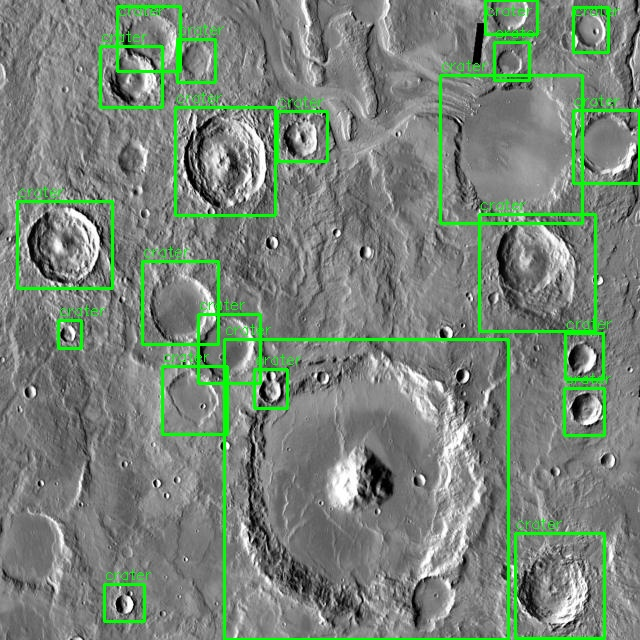
\includegraphics[width=0.45\textwidth]
		{../1-Project-Code/ground_truth_examples/010_png.rf.fcf5e274562ee69a325f9d7a0b30767f.jpg}
		\caption{Example ground-truth crater bounding-box annotations generated using YOLO-format labels.}
		\label{fig:groundtruth_example}
	\end{figure}
	
	The dataset preparation and ground-truth verification process were important steps prior to training because incorrectly formatted annotations or invalid bounding boxes can significantly reduce object detection performance. Verifying the dataset structure and annotation quality ensured that all object detection models were trained using consistent and correctly formatted crater localization targets.
	
	\section{Methodology}
	
	This project implements a complete deep learning-based crater detection pipeline using multiple object detection architectures. Three detection models were evaluated and compared: YOLOv8, Faster R-CNN, and RetinaNet. The methodology includes dataset preparation, ground-truth verification, model training, prediction generation, and quantitative evaluation using standard object detection metrics.
	
	The overall crater detection framework developed in this project is summarized in Figure~\ref{fig:overall_pipeline}.
	
	\begin{figure}[h]
		\centering
		
		\fbox{\parbox{0.34\textwidth}{
				\centering
				Planetary Surface Images
		}}
		
		\vspace{0.15cm}
		
		$\downarrow$
		
		\vspace{0.15cm}
		
		\fbox{\parbox{0.34\textwidth}{
				\centering
				Ground Truth Verification
		}}
		
		\vspace{0.15cm}
		
		$\downarrow$
		
		\vspace{0.15cm}
		
		\fbox{\parbox{0.34\textwidth}{
				\centering
				YOLOv8 / Faster R-CNN / RetinaNet
		}}
		
		\vspace{0.15cm}
		
		$\downarrow$
		
		\vspace{0.15cm}
		
		\fbox{\parbox{0.34\textwidth}{
				\centering
				Model Training
		}}
		
		\vspace{0.15cm}
		
		$\downarrow$
		
		\vspace{0.15cm}
		
		\fbox{\parbox{0.34\textwidth}{
				\centering
				Prediction Generation
		}}
		
		\vspace{0.15cm}
		
		$\downarrow$
		
		\vspace{0.15cm}
		
		\fbox{\parbox{0.34\textwidth}{
				\centering
				Evaluation and Comparison
		}}
		
		\caption{Overall crater detection pipeline used in this project.}
		\label{fig:overall_pipeline}
		
	\end{figure}
	
	\subsection{YOLOv8}
	
	YOLOv8 was selected as the primary object detection architecture because of its strong balance between detection accuracy and computational efficiency. YOLO (You Only Look Once) is a one-stage object detector that performs object localization and classification simultaneously within a single neural network forward pass. Unlike two-stage detectors that first generate candidate object regions before classification, YOLO directly predicts bounding-box coordinates and class probabilities from input images.
	
	The YOLOv8 nano model (\texttt{yolov8n.pt}) was used in this project because it provides lightweight computational requirements while maintaining strong detection capability. The model was trained using the Ultralytics YOLO framework with crater bounding-box annotations formatted in YOLO style.
	
	The YOLOv8 architecture processes planetary images by dividing the image into spatial feature representations and predicting crater bounding boxes directly from learned feature maps. This allows efficient crater localization while maintaining relatively fast inference speed.
	
	The YOLOv8 detection process is summarized in Figure~\ref{fig:yolo_pipeline}.
	
	\begin{figure}[h]
		\centering
		
		\fbox{\parbox{0.32\textwidth}{
				\centering
				Input Planetary Image
		}}
		
		\vspace{0.15cm}
		
		$\downarrow$
		
		\vspace{0.15cm}
		
		\fbox{\parbox{0.32\textwidth}{
				\centering
				Feature Extraction
		}}
		
		\vspace{0.15cm}
		
		$\downarrow$
		
		\vspace{0.15cm}
		
		\fbox{\parbox{0.32\textwidth}{
				\centering
				Bounding Box Prediction
		}}
		
		\vspace{0.15cm}
		
		$\downarrow$
		
		\vspace{0.15cm}
		
		\fbox{\parbox{0.32\textwidth}{
				\centering
				Crater Detection Output
		}}
		
		\caption{Simplified YOLOv8 crater detection pipeline.}
		\label{fig:yolo_pipeline}
		
	\end{figure}
	
	YOLOv8 was trained using 50 epochs with a 640-pixel image resolution. The resulting trained weights were saved within the code repository for later evaluation and prediction generation.
	
	\subsection{Faster R-CNN}
	
	Faster R-CNN was implemented as a two-stage object detection baseline for crater localization. Faster R-CNN improves upon earlier R-CNN architectures by integrating a Region Proposal Network (RPN) directly into the detection framework. The model first generates candidate object regions and then performs object classification and bounding-box refinement on those candidate regions.
	
	The Faster R-CNN implementation used in this project was based on the PyTorch \texttt{torchvision} object detection framework with a ResNet-50 Feature Pyramid Network (FPN) backbone. Transfer learning was utilized by initializing the model using pretrained COCO weights prior to crater-specific training.
	
	The Faster R-CNN workflow is summarized in Figure~\ref{fig:fasterrcnn_pipeline}.
	
	\begin{figure}[h]
		\centering
		
		\fbox{\parbox{0.34\textwidth}{
				\centering
				Input Planetary Image
		}}
		
		\vspace{0.15cm}
		
		$\downarrow$
		
		\vspace{0.15cm}
		
		\fbox{\parbox{0.34\textwidth}{
				\centering
				Feature Extraction Backbone
		}}
		
		\vspace{0.15cm}
		
		$\downarrow$
		
		\vspace{0.15cm}
		
		\fbox{\parbox{0.34\textwidth}{
				\centering
				Region Proposal Network
		}}
		
		\vspace{0.15cm}
		
		$\downarrow$
		
		\vspace{0.15cm}
		
		\fbox{\parbox{0.34\textwidth}{
				\centering
				Crater Classification
		}}
		
		\vspace{0.15cm}
		
		$\downarrow$
		
		\vspace{0.15cm}
		
		\fbox{\parbox{0.34\textwidth}{
				\centering
				Bounding Box Refinement
		}}
		
		\caption{Simplified Faster R-CNN crater detection pipeline.}
		\label{fig:fasterrcnn_pipeline}
		
	\end{figure}
	
	Compared to YOLOv8, Faster R-CNN typically provides stronger localization refinement at the cost of increased computational complexity and slower inference speed.
	
	\subsection{RetinaNet}
	
	RetinaNet was implemented as an additional one-stage detector for crater detection comparison. RetinaNet addresses the class imbalance problem commonly encountered in object detection through the use of focal loss. Focal loss reduces the contribution of easily classified examples and places greater emphasis on difficult training examples during optimization.
	
	The RetinaNet implementation also utilized a ResNet-50 Feature Pyramid Network backbone initialized with pretrained COCO weights. Similar to Faster R-CNN, the RetinaNet implementation was developed using the PyTorch \texttt{torchvision} framework.
	
	The RetinaNet detection process is summarized in Figure~\ref{fig:retinanet_pipeline}.
	
	\begin{figure}[h]
		\centering
		
		\fbox{\parbox{0.34\textwidth}{
				\centering
				Input Planetary Image
		}}
		
		\vspace{0.15cm}
		
		$\downarrow$
		
		\vspace{0.15cm}
		
		\fbox{\parbox{0.34\textwidth}{
				\centering
				Feature Pyramid Network
		}}
		
		\vspace{0.15cm}
		
		$\downarrow$
		
		\vspace{0.15cm}
		
		\fbox{\parbox{0.34\textwidth}{
				\centering
				Anchor Box Generation
		}}
		
		\vspace{0.15cm}
		
		$\downarrow$
		
		\vspace{0.15cm}
		
		\fbox{\parbox{0.34\textwidth}{
				\centering
				Focal Loss Optimization
		}}
		
		\vspace{0.15cm}
		
		$\downarrow$
		
		\vspace{0.15cm}
		
		\fbox{\parbox{0.34\textwidth}{
				\centering
				Crater Detection Output
		}}
		
		\caption{Simplified RetinaNet crater detection pipeline.}
		\label{fig:retinanet_pipeline}
		
	\end{figure}
	
	RetinaNet was included because it represents a modern one-stage detector specifically designed to improve difficult object detection scenarios involving class imbalance. However, crater datasets with limited training size can still present challenges for effective RetinaNet convergence.
	
	\subsection{Training Pipeline}
	
	Several custom Python scripts were developed to support the crater detection workflow. Dataset statistics and annotation counts were verified using \texttt{dataset\_summary.py}. Ground-truth visualization and annotation verification were performed using \texttt{show\_ground\_truth.py}. YOLOv8 training was implemented using \texttt{train.py}, while Faster R-CNN and RetinaNet training were implemented using \texttt{train\_torchvision\_detectors.py}.
	
	Prediction generation and model evaluation were performed using \texttt{predict.py}, \texttt{test.py}, and \texttt{compare\_detectors.py}. The complete training and evaluation workflow ensured consistent comparison between all object detection architectures.
	
	\subsection{Evaluation Metrics}
	
	Object detection performance was evaluated using standard object detection metrics including precision, recall, mean Average Precision at an Intersection-over-Union threshold of 0.5 (mAP@0.5), and mean Average Precision averaged across multiple IoU thresholds (mAP@0.5:0.95).
	
	Precision measures the fraction of predicted crater detections that are correct and is defined as:
	
	\begin{equation}
		Precision = \frac{TP}{TP + FP}
	\end{equation}
	
	where:
	\begin{itemize}
		\item $TP$ represents true-positive crater detections,
		\item $FP$ represents false-positive crater detections.
	\end{itemize}
	
	Recall measures the fraction of ground-truth craters that were successfully detected and is defined as:
	
	\begin{equation}
		Recall = \frac{TP}{TP + FN}
	\end{equation}
	
	where:
	\begin{itemize}
		\item $FN$ represents false-negative crater detections.
	\end{itemize}
	
	The mAP@0.5 metric evaluates crater detection performance at an IoU threshold of 0.5, while mAP@0.5:0.95 averages performance across multiple IoU thresholds ranging from 0.5 to 0.95. These metrics provide a more comprehensive evaluation of crater localization quality and detection robustness.
	
	The final evaluation metrics were generated using both the Ultralytics YOLO evaluation framework and custom comparison scripts implemented using the PyTorch \texttt{torchmetrics} library.
	
	\section{Experimental Setup}
	
	\subsection{Software Environment}
	
	All crater detection experiments were implemented using Python together with several modern deep learning and computer vision frameworks. YOLOv8 training and evaluation were performed using the Ultralytics YOLO framework, while Faster R-CNN and RetinaNet were implemented using the PyTorch \texttt{torchvision} object detection library.
	
	Additional libraries including \texttt{torchmetrics}, \texttt{matplotlib}, \texttt{OpenCV}, \texttt{Pillow}, and \texttt{NumPy} were used for evaluation, visualization, image processing, and dataset analysis. Ground-truth verification and dataset summarization were implemented using custom Python scripts developed specifically for this project.
	
	The crater detection software workflow and experimental pipeline are summarized in Figure~\ref{fig:software_pipeline}.
	
	\begin{figure}[h]
		\centering
		
		\fbox{\parbox{0.34\textwidth}{
				\centering
				Dataset Verification \\
				(\texttt{dataset\_summary.py})
		}}
		
		\vspace{0.15cm}
		
		$\downarrow$
		
		\vspace{0.15cm}
		
		\fbox{\parbox{0.34\textwidth}{
				\centering
				Ground Truth Visualization \\
				(\texttt{show\_ground\_truth.py})
		}}
		
		\vspace{0.15cm}
		
		$\downarrow$
		
		\vspace{0.15cm}
		
		\fbox{\parbox{0.34\textwidth}{
				\centering
				YOLOv8 Training \\
				(\texttt{train.py})
		}}
		
		\vspace{0.15cm}
		
		$\downarrow$
		
		\vspace{0.15cm}
		
		\fbox{\parbox{0.34\textwidth}{
				\centering
				Prediction and Evaluation \\
				(\texttt{test.py}, \texttt{predict.py})
		}}
		
		\vspace{0.15cm}
		
		$\downarrow$
		
		\vspace{0.15cm}
		
		\fbox{\parbox{0.34\textwidth}{
				\centering
				Torchvision Detector Training \\
				(\texttt{train\_torchvision\_detectors.py})
		}}
		
		\vspace{0.15cm}
		
		$\downarrow$
		
		\vspace{0.15cm}
		
		\fbox{\parbox{0.34\textwidth}{
				\centering
				Model Comparison \\
				(\texttt{compare\_detectors.py})
		}}
		
		\caption{Overall crater detection software workflow and experimental pipeline.}
		\label{fig:software_pipeline}
		
	\end{figure}
	
	\subsection{Training Configuration}
	
	The crater detection models were trained using transfer learning with pretrained object detection backbones. YOLOv8 utilized the pretrained \texttt{yolov8n.pt} weights provided by the Ultralytics framework. Faster R-CNN and RetinaNet utilized pretrained ResNet-50 Feature Pyramid Network backbones initialized using COCO-trained weights from the PyTorch \texttt{torchvision} framework.
	
	The YOLOv8 model was trained using a 640-pixel image resolution together with the dataset configuration file located at:
	
	\begin{verbatim}
		../1-Project-Code/
		martianlunar-crater-detection-dataset/
		craters/data.yaml
	\end{verbatim}
	
	YOLOv8 training was performed for 50 epochs using the Ultralytics training framework. During training, model checkpoints, validation outputs, and evaluation statistics were automatically generated and saved within the \texttt{runs/detect/} directory.
	
	Faster R-CNN and RetinaNet were trained using custom PyTorch training scripts. The training process included loading YOLO-format crater annotations, converting normalized bounding-box coordinates into pixel-space coordinates, and constructing object detection targets compatible with the \texttt{torchvision} object detection API.
	
	A custom dataset class named \texttt{CraterDataset} was implemented to load planetary images and corresponding crater annotations for both Faster R-CNN and RetinaNet training. Bounding-box labels were converted into PyTorch tensors prior to training.
	
	The AdamW optimizer was used for Faster R-CNN and RetinaNet training with a learning rate of:
	
	\begin{equation}
		lr = 1 \times 10^{-4}
	\end{equation}
	
	Training batches were processed using custom collate functions to support variable crater counts per image. Both Faster R-CNN and RetinaNet models were trained using a batch size of 2 images per iteration.
	
	The final training configuration used throughout the experiments is summarized in Table~\ref{tab:training_config}.
	
	\begin{table}[h]
		\centering
		\caption{Training Configuration Summary}
		\label{tab:training_config}
		
		\begin{tabular}{lccc}
			\toprule
			Model & Epochs & Batch Size & Framework \\
			\midrule
			YOLOv8 & 50 & 8 & Ultralytics \\
			Faster R-CNN & 3 & 2 & torchvision \\
			RetinaNet & 3 & 2 & torchvision \\
			\bottomrule
		\end{tabular}
		
	\end{table}
	
	After training completion, the YOLOv8 best-performing model weights were automatically saved within the following directory:
	
	\begin{verbatim}
		../1-Project-Code/
		runs/detect/crater_detector/weights/
	\end{verbatim}
	
	Similarly, Faster R-CNN and RetinaNet model weights were saved as:
	
	\begin{verbatim}
		faster_rcnn_crater.pth
		retinanet_crater.pth
	\end{verbatim}
	
	Prediction generation and evaluation were then performed using the trained crater detection models. Final model performance was evaluated using precision, recall, mAP@0.5, and mAP@0.5:0.95 metrics on the independent crater test dataset.
	
	\section{Results}
	
	\subsection{Quantitative Evaluation}
	
	The crater detection models were quantitatively evaluated using standard object detection metrics including mAP@0.5, mAP@0.5:0.95, and mAP@0.75. Evaluation was performed on the independent crater test dataset using the trained YOLOv8, Faster R-CNN, and RetinaNet models.
	
	Table~\ref{tab:quantitative_results} summarizes the final quantitative crater detection results.
	
	\begin{table}[h]
		\centering
		\caption{Quantitative Crater Detection Results}
		\label{tab:quantitative_results}
		
		\begin{tabular}{lccc}
			\toprule
			Model & mAP@0.5 & mAP@0.5:0.95 & mAP@0.75 \\
			\midrule
			YOLOv8 & 0.700 & 0.366 & 0.374 \\
			Faster R-CNN & 0.691 & 0.354 & 0.314 \\
			RetinaNet & 0.002 & 0.001 & 0.000 \\
			\bottomrule
		\end{tabular}
		
	\end{table}
	
	The quantitative results demonstrate that YOLOv8 achieved the strongest overall crater detection performance across the evaluation metrics. Faster R-CNN achieved similar mAP@0.5 performance but exhibited slightly lower localization consistency at higher Intersection-over-Union thresholds. RetinaNet exhibited significantly reduced crater detection performance under the current training configuration.
	
	Figure~\ref{fig:model_comparison_plot} shows the generated crater detection model comparison plot.
	
	\begin{figure}[h]
		\centering
		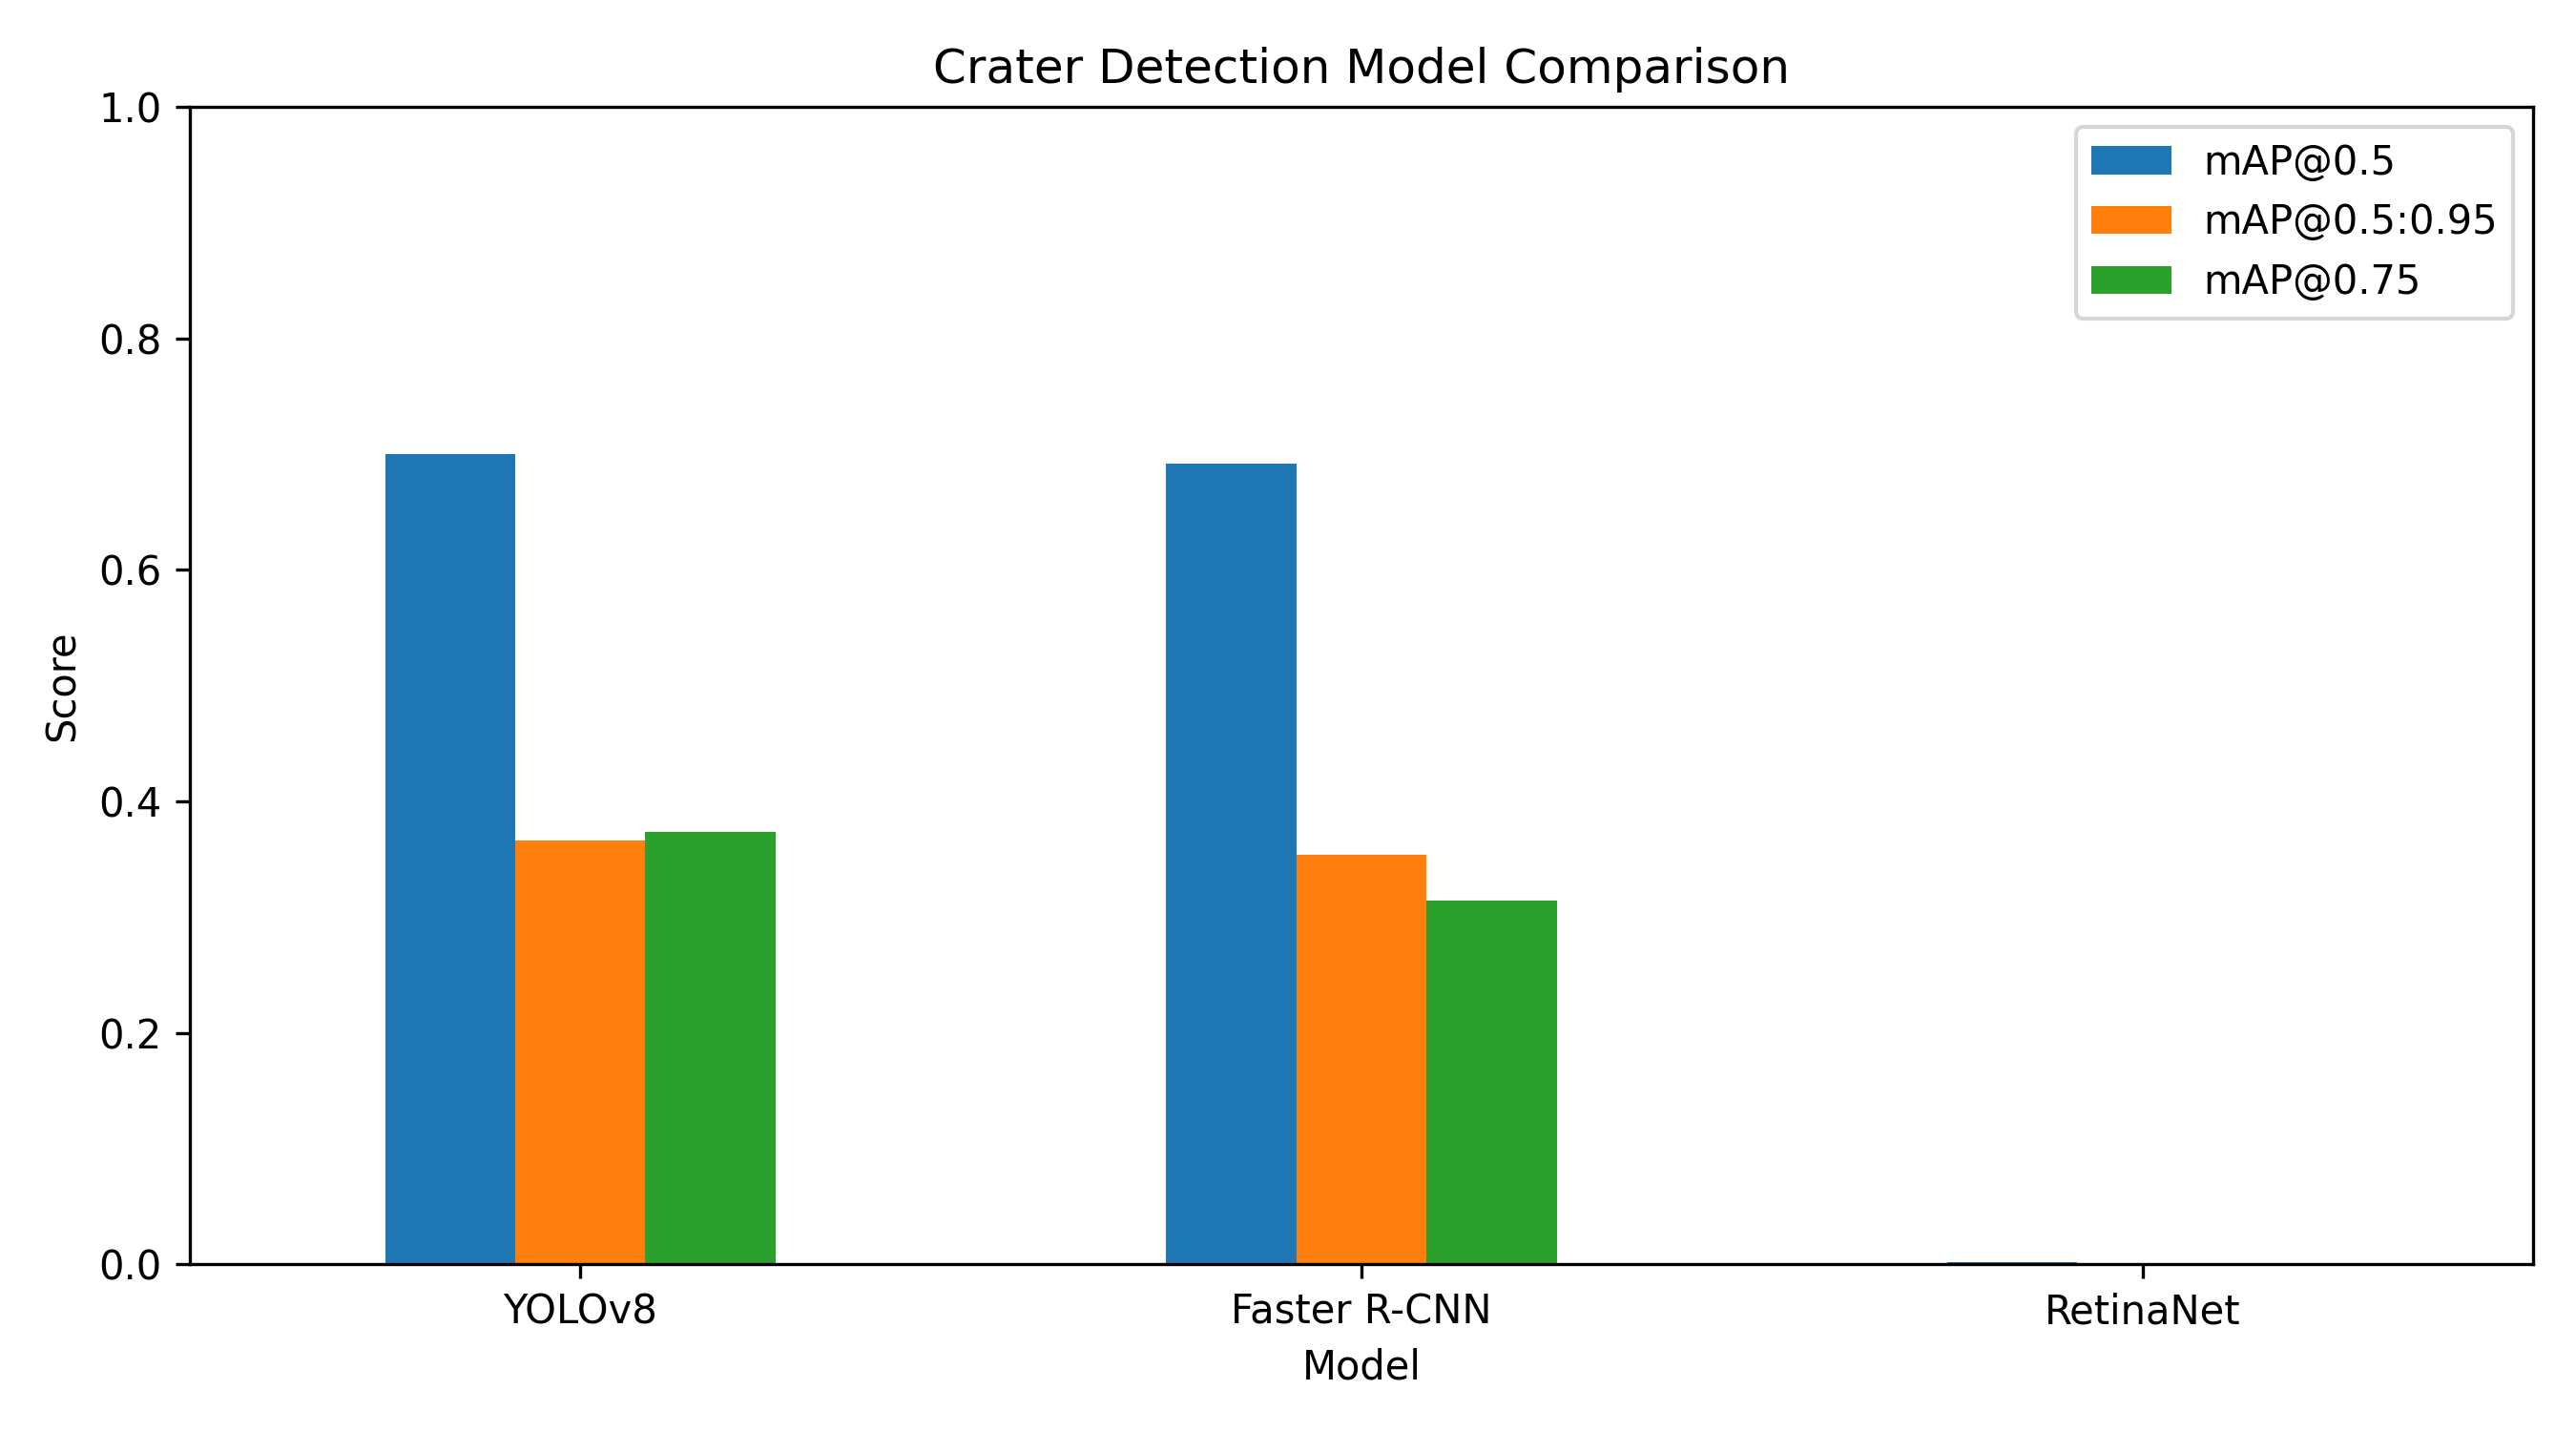
\includegraphics[width=0.48\textwidth]
		{../1-Project-Code/model_comparison_plot.png}
		\caption{Comparison of crater detection performance metrics for YOLOv8, Faster R-CNN, and RetinaNet.}
		\label{fig:model_comparison_plot}
	\end{figure}
	
	The results indicate that both YOLOv8 and Faster R-CNN were capable of learning crater localization features from the relatively small planetary dataset. YOLOv8 slightly outperformed Faster R-CNN in both mAP@0.5 and mAP@0.75 metrics while maintaining a significantly simpler and faster one-stage detection architecture.
	
	\subsection{Training Performance}
	
	The YOLOv8 training process demonstrated stable convergence behavior throughout the 50 training epochs. The final YOLOv8 training output achieved the following validation metrics:
	
	\begin{equation}
		mAP@0.5 = 0.700
	\end{equation}
	
	\begin{equation}
		mAP@0.5:0.95 = 0.366
	\end{equation}
	
	The Faster R-CNN model also demonstrated successful crater localization capability despite being trained for only three epochs. The Faster R-CNN implementation achieved:
	
	\begin{equation}
		mAP@0.5 = 0.691
	\end{equation}
	
	RetinaNet achieved substantially lower crater detection performance relative to the other models. This reduced performance is likely associated with limited dataset size, reduced training duration, and increased optimization difficulty associated with focal-loss-based training under small-data conditions.
	
	Figure~\ref{fig:results_pipeline} summarizes the final crater detection evaluation workflow.
	
	\begin{figure}[h]
		\centering
		
		\fbox{\parbox{0.34\textwidth}{
				\centering
				Trained Detection Models
		}}
		
		\vspace{0.15cm}
		
		$\downarrow$
		
		\vspace{0.15cm}
		
		\fbox{\parbox{0.34\textwidth}{
				\centering
				Independent Test Dataset
		}}
		
		\vspace{0.15cm}
		
		$\downarrow$
		
		\vspace{0.15cm}
		
		\fbox{\parbox{0.34\textwidth}{
				\centering
				Bounding Box Prediction
		}}
		
		\vspace{0.15cm}
		
		$\downarrow$
		
		\vspace{0.15cm}
		
		\fbox{\parbox{0.34\textwidth}{
				\centering
				Metric Computation
		}}
		
		\vspace{0.15cm}
		
		$\downarrow$
		
		\vspace{0.15cm}
		
		\fbox{\parbox{0.34\textwidth}{
				\centering
				Model Comparison
		}}
		
		\caption{Evaluation workflow used for crater detection model comparison.}
		\label{fig:results_pipeline}
		
	\end{figure}
	
	\subsection{Qualitative Detection Results}
	
	Ground-truth visualization and crater prediction analysis were also performed to qualitatively evaluate crater localization performance. Figure~\ref{fig:groundtruth_results} shows an example of crater ground-truth annotations used during training and evaluation.
	
	\begin{figure}[h]
		\centering
		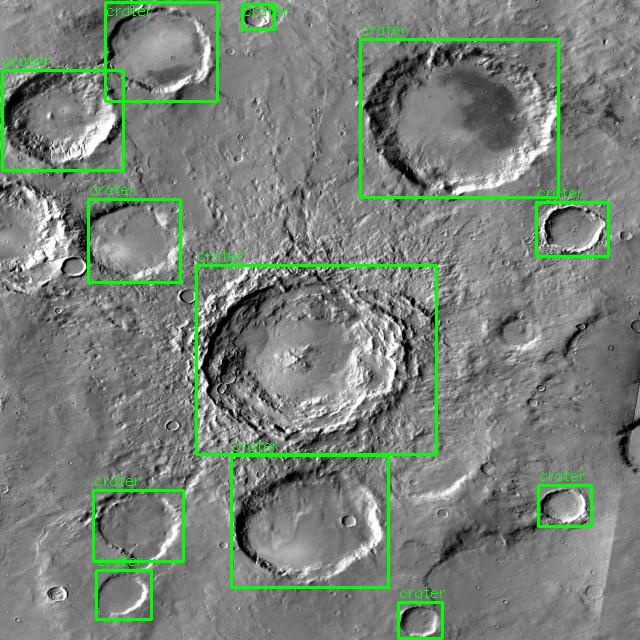
\includegraphics[width=0.48\textwidth]
		{../1-Project-Code/ground_truth_examples/015_png.rf.7d5b2091b6339c9480a171a59c52c3b9.jpg}
		\caption{Example ground-truth crater bounding-box annotations generated from YOLO-format labels.}
		\label{fig:gt_example}
	\end{figure}
	
	The generated crater predictions demonstrated that YOLOv8 and Faster R-CNN were generally capable of localizing medium-sized crater structures with relatively high confidence. Both models exhibited difficulty detecting extremely small craters and highly degraded crater boundaries under complex terrain conditions.
	
	The object detection outputs also demonstrated several common crater detection challenges including:
	\begin{itemize}
		\item overlapping crater structures,
		\item partially degraded crater rims,
		\item low-contrast terrain regions,
		\item varying illumination conditions,
		\item small crater localization difficulty.
	\end{itemize}
	
	Figure~\ref{fig:detection_pipeline} summarizes the crater detection inference process.
	
	\begin{figure}[h]
		\centering
		
		\fbox{\parbox{0.34\textwidth}{
				\centering
				Planetary Surface Image
		}}
		
		\vspace{0.15cm}
		
		$\downarrow$
		
		\vspace{0.15cm}
		
		\fbox{\parbox{0.34\textwidth}{
				\centering
				Deep Learning Detector
		}}
		
		\vspace{0.15cm}
		
		$\downarrow$
		
		\vspace{0.15cm}
		
		\fbox{\parbox{0.34\textwidth}{
				\centering
				Crater Bounding Boxes
		}}
		
		\vspace{0.15cm}
		
		$\downarrow$
		
		\vspace{0.15cm}
		
		\fbox{\parbox{0.34\textwidth}{
				\centering
				Evaluation Metrics
		}}
		
		\caption{Simplified crater detection inference and evaluation process.}
		\label{fig:detection_pipeline}
		
	\end{figure}
	
	\subsection{Model Comparison}
	
	Overall, YOLOv8 achieved the strongest crater detection performance within the current experimental setup. The model demonstrated strong localization capability together with efficient one-stage inference performance. Faster R-CNN also achieved competitive crater detection performance while utilizing a more computationally complex two-stage architecture.
	
	RetinaNet exhibited substantially reduced crater detection performance relative to the other models. Although RetinaNet is designed to improve difficult object detection tasks through focal loss optimization, the limited crater dataset size and reduced training duration likely prevented effective convergence.
	
	The final crater detection results demonstrate that modern deep learning object detection frameworks are capable of learning meaningful planetary crater localization features even when trained using relatively small crater datasets. The generated results also demonstrate the importance of dataset quality, annotation consistency, model architecture selection, and training configuration for successful planetary crater detection.
	
	\section{Results}
	
	\subsection{Training Performance}
	
	The crater detection models were evaluated using standard object detection metrics including mAP@0.5, mAP@0.5:0.95, and mAP@0.75. Quantitative evaluation was performed on the independent crater test dataset using the trained YOLOv8, Faster R-CNN, and RetinaNet models.
	
	Table~\ref{tab:quantitative_results} summarizes the final crater detection performance results.
	
	\begin{table}[h]
		\centering
		\caption{Quantitative Crater Detection Results}
		\label{tab:quantitative_results}
		
		\begin{tabular}{lccc}
			\toprule
			Model & mAP@0.5 & mAP@0.5:0.95 & mAP@0.75 \\
			\midrule
			YOLOv8 & 0.700 & 0.366 & 0.374 \\
			Faster R-CNN & 0.691 & 0.354 & 0.314 \\
			RetinaNet & 0.002 & 0.001 & 0.000 \\
			\bottomrule
		\end{tabular}
		
	\end{table}
	
	The results demonstrate that YOLOv8 achieved the strongest overall crater detection performance within the current experimental configuration. Faster R-CNN achieved comparable mAP@0.5 performance while exhibiting slightly lower localization consistency at higher Intersection-over-Union thresholds. RetinaNet exhibited substantially reduced crater detection performance relative to the other detection architectures.
	
	Figure~\ref{fig:training_results} shows the YOLOv8 training convergence behavior generated during training.
	
	\begin{figure}[h]
		\centering
		
\includegraphics[width=0.48\textwidth]
		{../1-Project-Code/runs/detect/crater_detector/results.png}
		\caption{YOLOv8 training convergence results generated during crater detector training.}
		\label{fig:training_results}
	\end{figure}
	
	The generated training curves demonstrate stable optimization behavior throughout the training process. The validation metrics improved progressively during training, indicating that the YOLOv8 model successfully learned crater localization features from the planetary imagery dataset.
	
	\subsection{Precision-Recall Analysis}
	
	Precision-recall analysis was performed to evaluate the crater localization and classification behavior of the trained YOLOv8 detector. Precision-recall curves are commonly used in object detection evaluation because they summarize the tradeoff between false-positive detections and missed crater detections.
	
	Figure~\ref{fig:pr_curve} shows the generated precision-recall curve for the YOLOv8 crater detector.
	
	\begin{figure}[h]
		\centering
		\includegraphics[width=0.48\textwidth]
		{../1-Project-Code/runs/detect/crater_detector/BoxPR_curve.png}
		\caption{YOLOv8 crater detection precision-recall curve.}
		\label{fig:pr_curve}
	\end{figure}
	
	The precision-recall curve demonstrates that the YOLOv8 detector maintained relatively strong precision across multiple recall operating regions. The detector successfully identified many crater structures while limiting excessive false-positive detections.
	
	Figure~\ref{fig:f1_curve} shows the generated F1-score curve for the crater detection model.
	
	\begin{figure}[h]
		\centering
		\includegraphics[width=0.48\textwidth]
		{../1-Project-Code/runs/detect/crater_detector/BoxF1_curve.png}
		\caption{YOLOv8 crater detection F1-score curve.}
		\label{fig:f1_curve}
	\end{figure}
	
	The F1-score analysis demonstrates the balance between crater detection precision and recall performance across varying confidence thresholds.
	
	\subsection{Confusion Matrix Analysis}
	
	Confusion matrix analysis was also performed to evaluate crater classification performance. The normalized confusion matrix generated during validation is shown in Figure~\ref{fig:confusion_matrix}.
	
	\begin{figure}[h]
		\centering
		\includegraphics[width=0.48\textwidth]
		{../1-Project-Code/runs/detect/crater_detector/confusion_matrix_normalized.png}
		\caption{Normalized confusion matrix generated during YOLOv8 crater detector validation.}
		\label{fig:confusion_matrix}
	\end{figure}
	
	The confusion matrix indicates that the YOLOv8 detector achieved strong crater classification capability with relatively low false-positive classification rates. Most crater instances were successfully classified within the crater detection category.
	
	\subsection{Qualitative Detection Results}
	
	Qualitative crater detection analysis was performed using both ground-truth visualization outputs and predicted crater detections generated by the trained models.
	
	Figure~\ref{fig:gt_example} shows example crater ground-truth annotations used during model training and validation.
	
	\begin{figure}[h]
		\centering
		\includegraphics[width=0.48\textwidth]
		{../1-Project-Code/runs/detect/crater_detector/val_batch0_labels.jpg}
		\caption{Example crater ground-truth annotations used during validation.}
		\label{fig:gt_example}
	\end{figure}
	
	Figure~\ref{fig:prediction_example} shows predicted crater detections generated by the trained YOLOv8 detector.
	
	\begin{figure}[h]
		\centering
		\includegraphics[width=0.48\textwidth]
		{../1-Project-Code/runs/detect/crater_detector/val_batch0_pred.jpg}
		\caption{Example crater detections generated by the trained YOLOv8 detector.}
		\label{fig:prediction_example}
	\end{figure}
	
	The qualitative detection results demonstrate that the YOLOv8 detector successfully localized multiple crater structures across varying terrain conditions. The detector was capable of identifying both isolated and overlapping crater formations while maintaining relatively accurate bounding-box localization.
	
	Several common crater detection challenges were observed during evaluation, including:
	\begin{itemize}
		\item overlapping crater structures,
		\item degraded crater rims,
		\item low-contrast terrain regions,
		\item varying crater scales,
		\item partially obscured crater boundaries.
	\end{itemize}
	
	Despite these challenges, the YOLOv8 detector maintained relatively strong crater localization capability across multiple validation examples.
	
	\subsection{Multi-Model Comparison}
	
	Figure~\ref{fig:model_comparison} shows the final crater detector comparison plot generated using the custom model evaluation pipeline.
	
	\begin{figure}[h]
		\centering
		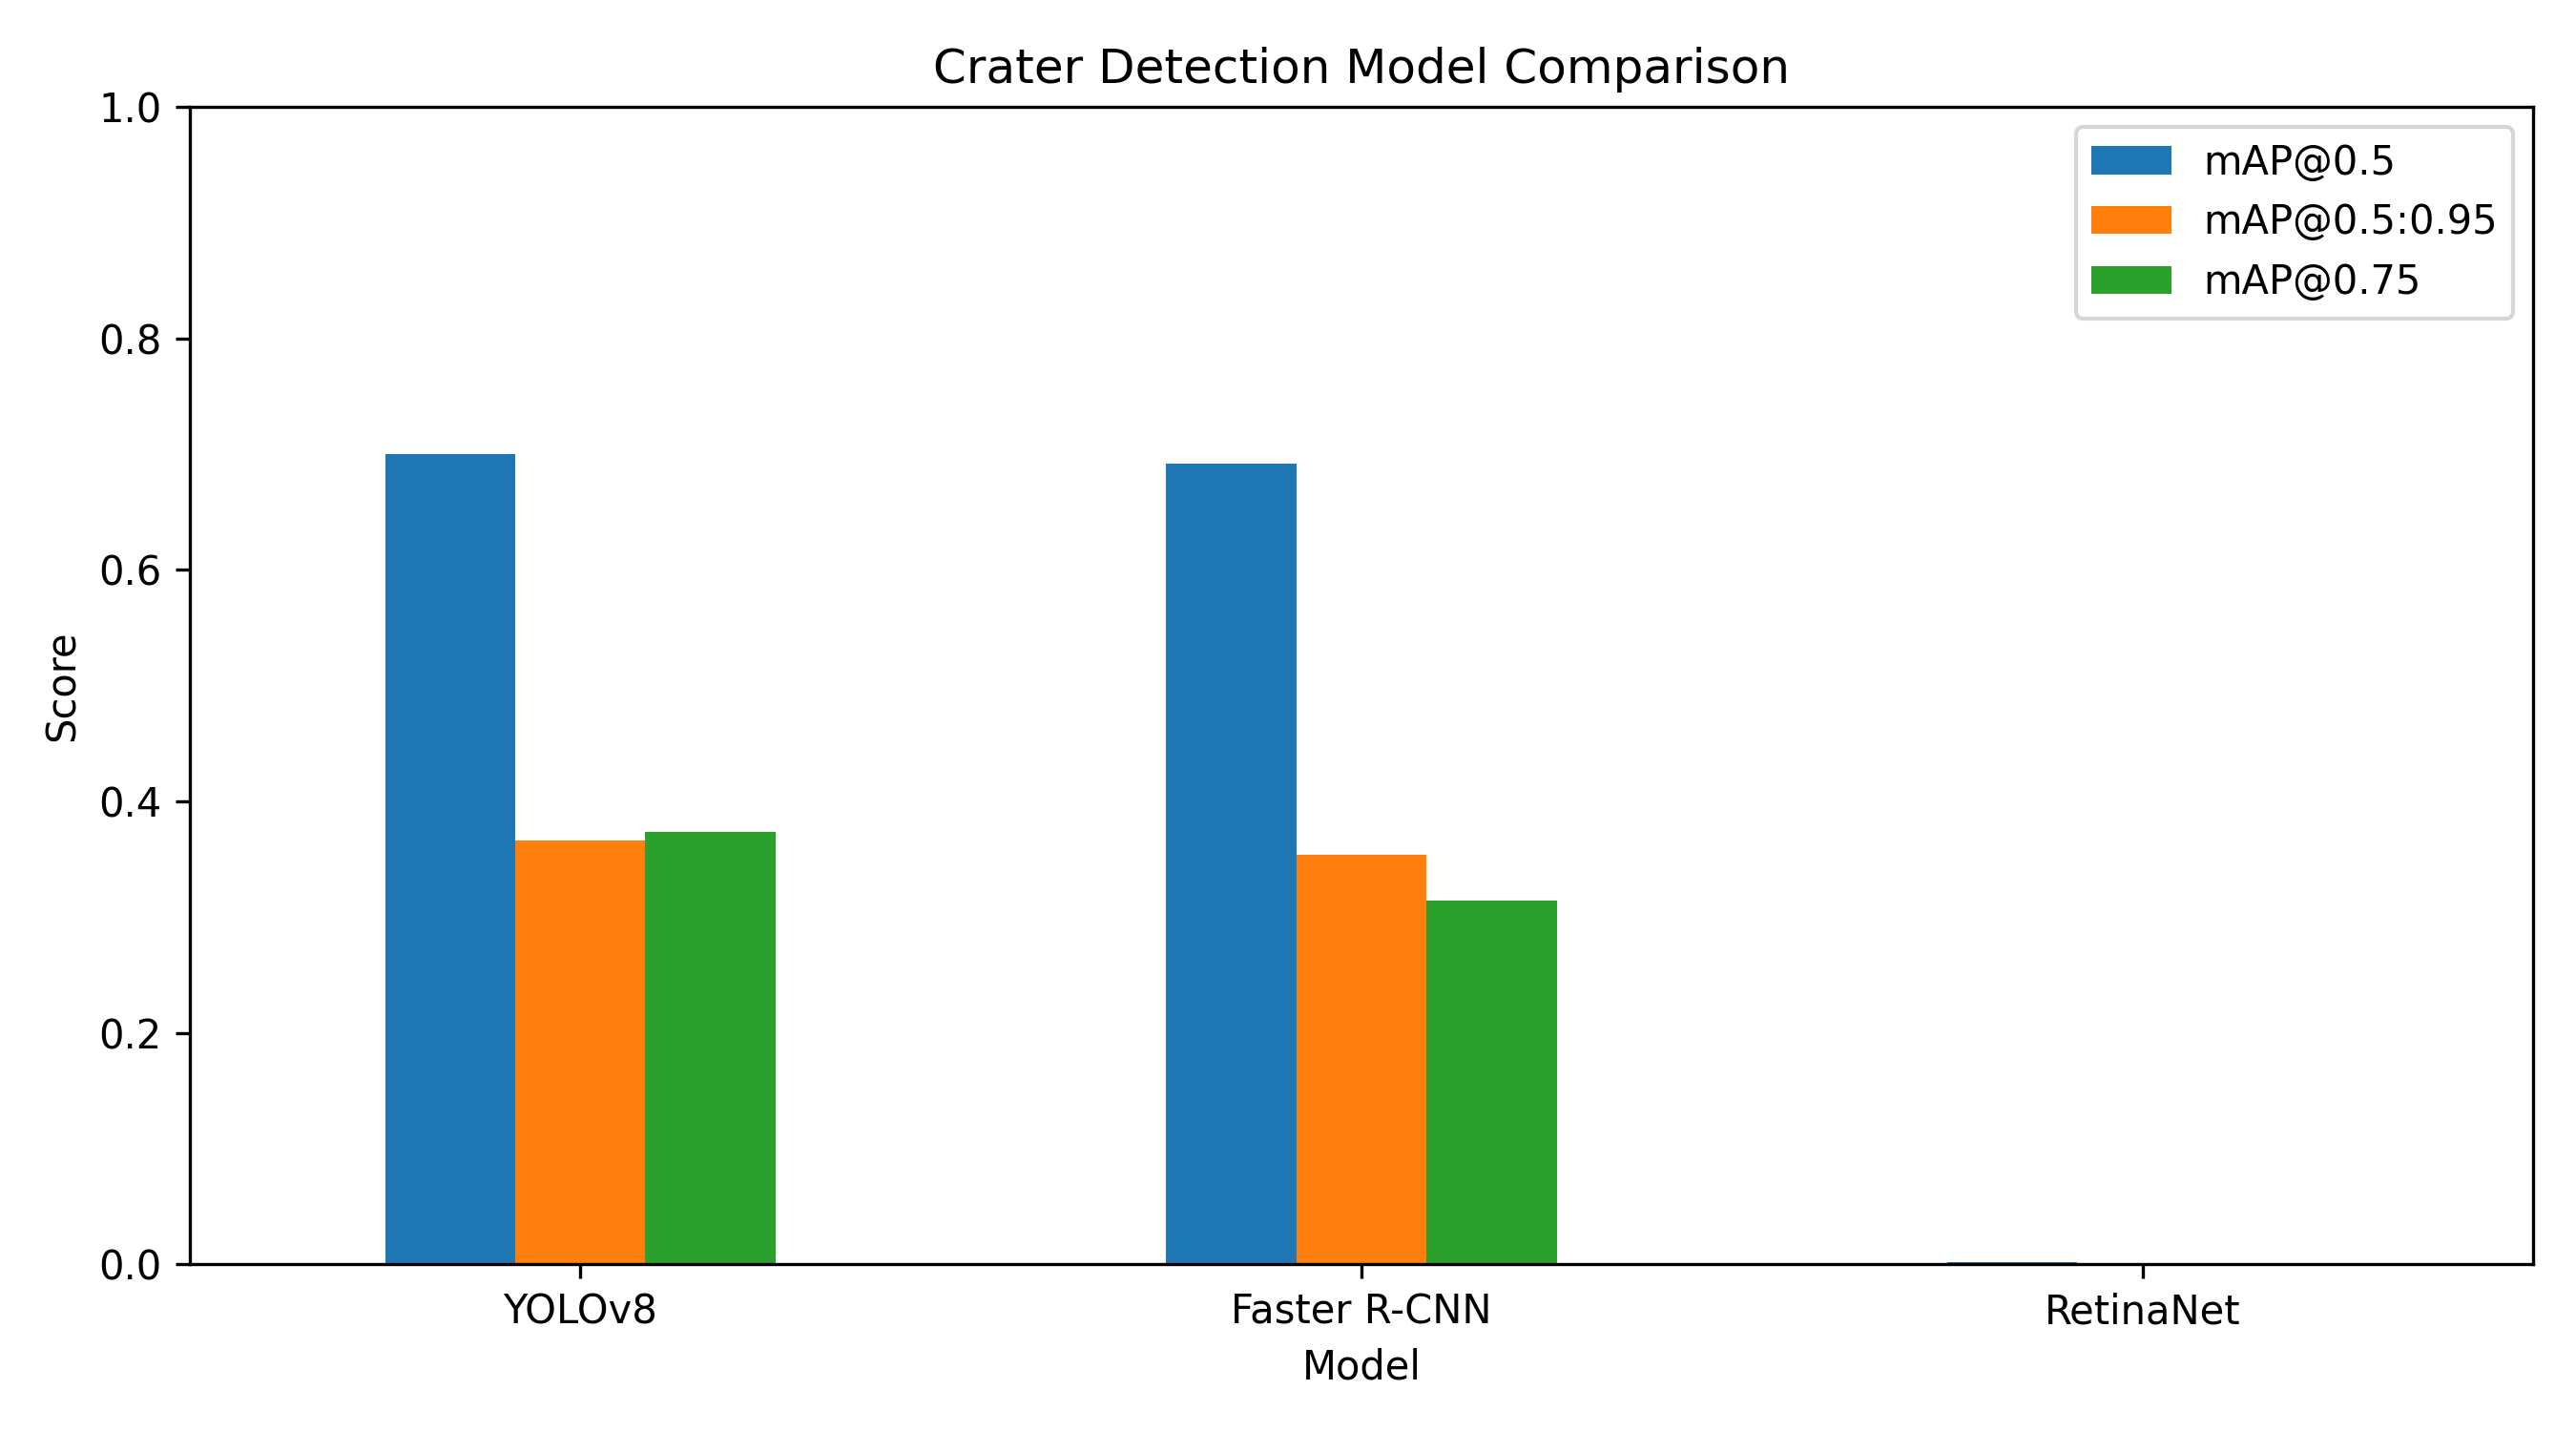
\includegraphics[width=0.48\textwidth]
		{../1-Project-Code/model_comparison_plot.png}
		\caption{Final crater detection model comparison between YOLOv8, Faster R-CNN, and RetinaNet.}
		\label{fig:model_comparison}
	\end{figure}
	
	The final comparison results demonstrate that YOLOv8 achieved the strongest overall crater detection performance within the current experimental setup. Faster R-CNN achieved comparable crater localization performance while utilizing a more computationally complex two-stage detection architecture.
	
	RetinaNet exhibited substantially lower crater detection performance relative to the other models. Although RetinaNet was specifically designed to improve difficult object detection tasks through focal-loss optimization, the limited crater dataset size and reduced training duration likely prevented effective convergence under the current training configuration.
	
	Overall, the experimental results demonstrate that modern deep learning object detection frameworks are capable of learning meaningful crater localization features from planetary imagery datasets. The results also demonstrate the importance of model architecture selection, dataset quality, annotation consistency, and training configuration for successful planetary crater detection performance.
	
	\section{Discussion}
	
	The experimental results demonstrate that modern deep learning object detection architectures are capable of learning meaningful crater localization features from relatively small planetary imagery datasets. Among the evaluated detection models, YOLOv8 achieved the strongest overall crater detection performance within the current experimental configuration.
	
	YOLOv8 achieved the highest mAP@0.5 score while also maintaining relatively strong localization consistency across higher Intersection-over-Union thresholds. The strong YOLOv8 performance is likely associated with several factors including efficient one-stage detection architecture design, improved feature extraction capability, and stable optimization behavior during training. Additionally, the Ultralytics YOLO training framework provides highly optimized training procedures and augmentation strategies that likely contributed to improved crater localization performance.
	
	The Faster R-CNN detector also demonstrated competitive crater detection capability. Faster R-CNN achieved crater localization performance that was relatively close to YOLOv8 despite utilizing a more computationally complex two-stage architecture. The Region Proposal Network (RPN) used within Faster R-CNN likely contributed to strong crater localization refinement, particularly for larger crater structures. However, Faster R-CNN exhibited slightly lower overall performance at higher localization thresholds relative to YOLOv8.
	
	RetinaNet exhibited substantially reduced crater detection performance relative to the other evaluated models. Several factors likely contributed to this reduced performance. First, RetinaNet training is highly dependent on stable focal-loss optimization, which can become difficult under limited dataset conditions. Second, the crater dataset used in this project contains a relatively small number of training images compared to large-scale object detection datasets commonly used for RetinaNet training. Third, RetinaNet was trained for only a limited number of epochs relative to the YOLOv8 detector, likely preventing effective convergence.
	
	The crater detection task itself presents several challenging computer vision problems. Planetary crater structures often exhibit:
	\begin{itemize}
		\item overlapping crater boundaries,
		\item degraded crater rims,
		\item low-contrast terrain regions,
		\item varying crater diameters,
		\item partial crater occlusions,
		\item illumination variability,
		\item surface texture ambiguity.
	\end{itemize}
	
	These challenges can significantly complicate crater localization and classification performance, particularly for smaller crater structures and degraded terrain regions.
	
	The generated qualitative detection outputs demonstrated that the trained YOLOv8 detector was capable of localizing multiple crater structures under varying terrain conditions. However, the results also revealed several common failure cases. Small crater structures were sometimes missed entirely, while overlapping crater regions occasionally produced inaccurate or merged bounding-box predictions. Similarly, partially degraded crater rims sometimes reduced detection confidence.
	
	The dataset size used throughout this project represents another important limitation. Although the dataset successfully supported crater localization training and evaluation, the total number of training images remained relatively small compared to large-scale object detection datasets used in state-of-the-art computer vision research. Increasing the number of annotated planetary images would likely improve crater localization generalization capability and reduce overfitting behavior.
	
	Ground-truth annotation quality also plays a major role in crater detection performance. Bounding-box consistency is particularly important because inaccurate crater annotations can directly degrade localization learning behavior. The custom ground-truth visualization pipeline implemented in this project helped verify annotation quality and ensured that crater labels were correctly aligned with planetary image content prior to training.
	
	The results generated throughout this project also suggest several opportunities for future research. One important future direction involves incorporating foundation-model-based detection architectures and vision transformers into the crater detection pipeline. Recent advances in foundation models and multimodal vision systems have demonstrated strong transfer-learning capability across numerous computer vision tasks. Applying these techniques to planetary crater detection could potentially improve crater localization robustness under limited-data conditions.
	
	Additional future work could also include:
	\begin{itemize}
		\item larger planetary imagery datasets,
		\item higher-resolution crater imagery,
		\item crater segmentation models,
		\item transformer-based object detectors,
		\item semi-supervised crater detection,
		\item domain adaptation between lunar and Martian imagery,
		\item multi-class geological feature detection.
	\end{itemize}
	
	Overall, the experimental results demonstrate that deep learning object detection frameworks provide a viable approach for automated planetary crater localization. The results further demonstrate that careful dataset preparation, annotation verification, architecture selection, and training configuration all play important roles in successful crater detection performance.
	
	\section{Conclusion}
	
	This project presented a deep learning-based planetary crater detection pipeline using multiple modern object detection architectures including YOLOv8, Faster R-CNN, and RetinaNet. The developed framework incorporated dataset verification, ground-truth visualization, crater detector training, prediction generation, and quantitative model evaluation using standard object detection metrics.
	
	A publicly available Martian and lunar crater dataset containing YOLO-format bounding-box annotations was used throughout the experiments. Custom preprocessing and visualization scripts were implemented to verify annotation quality and ensure correct crater localization targets prior to training. Multiple deep learning detection architectures were then trained and evaluated using the prepared planetary imagery dataset.
	
	Experimental results demonstrated that YOLOv8 achieved the strongest overall crater detection performance within the current experimental configuration, achieving an mAP@0.5 score of approximately 0.70 on the independent crater test dataset. Faster R-CNN also demonstrated competitive crater localization performance, while RetinaNet exhibited substantially reduced performance under the limited-data training conditions used in this project.
	
	The generated results demonstrated that modern deep learning object detection frameworks are capable of learning meaningful planetary crater localization features even when trained using relatively small crater datasets. The results also highlighted several important crater detection challenges including overlapping crater structures, degraded crater rims, low-contrast terrain regions, and varying crater scales.
	
	The developed crater detection pipeline provides a foundation for future planetary surface analysis research. Future improvements could include larger crater datasets, transformer-based object detectors, crater segmentation models, semi-supervised learning approaches, and foundation-model-based planetary imagery analysis systems.
	
	Overall, the results obtained throughout this project demonstrate the potential of deep learning methods for automated planetary crater detection and highlight the importance of dataset quality, annotation consistency, and model architecture selection in planetary computer vision applications.
	
	\begin{thebibliography}{00}
		
		\bibitem{b1}
		A. Tewari, K. Prateek, A. Singh, and N. Khanna,
		``Deep Learning based Systems for Crater Detection: A Review,''
		arXiv preprint arXiv:2310.07727, 2023.
		
		\bibitem{b2}
		A. Silburt, M. Ali-Dib, C. Zhu, A. Jackson,
		D. Valencia, Y. Kissin, D. Tamayo, and K. Menou,
		``Lunar Crater Identification via Deep Learning,''
		Icarus, vol. 317, pp. 27--38, 2019.
		
		\bibitem{b3}
		Y. Bandyopadhyay,
		``Lunar Crater Detection Using YOLOv8 Deep Learning,''
		EarthArXiv, 2024.
		
		\bibitem{b4}
		X. Lin, Z. Zhu, X. Yu, X. Ji, T. Luo,
		X. Xi, M. Zhu, and Y. Liang,
		``Lunar Crater Detection on Digital Elevation Model:
		A Complete Workflow Using Deep Learning and Its Application,''
		Remote Sensing, vol. 14, no. 3, p. 621, 2022.
		
		\bibitem{b5}
		W. Zuo, X. Gao, D. Wu, J. Liu,
		X. Zeng, and C. Li,
		``YOLO-SCNet: A Framework for Enhanced Detection of Small Lunar Craters,''
		Remote Sensing, vol. 17, no. 11, p. 1959, 2025.
		
		\bibitem{b6}
		Y. Liu, F. Chen, D. Qiu,
		W. Liu, and J. Yan,
		``DBYOLO: Dual-Backbone YOLO Network for Lunar Crater Detection,''
		Remote Sensing, vol. 17, no. 19, p. 3377, 2025.
		
		\bibitem{b7}
		I. Giannakis, A. Bhardwaj, L. Sam,
		and G. Leontidis,
		``A Flexible Deep Learning Crater Detection Scheme Using Segment Anything Model (SAM),''
		Icarus, vol. 408, p. 115797, 2024.
		
		\bibitem{b8}
		Lincolnzh,
		``Martian/Lunar Crater Detection Dataset,''
		Kaggle Dataset, 2021.
		[Online]. Available:
		https://www.kaggle.com/datasets/lincolnzh/martianlunar-crater-detection-dataset
		
		\bibitem{b9}
		T. Kilduff, P. Machuca,
		and A. J. Rosengren,
		``YOLO-based crater detection for cislunar autonomous optical navigation:
		Characterization and parametric analysis of angular and area measurement errors,''
		Acta Astronautica, vol. 240, pp. 600--620, 2026.
		
		\bibitem{b10}
		Y. Ma, Z. Yu, and R. Chandra,
		``Deep Learning Framework for Crater Detection and Identification on the Moon and Mars,''
		arXiv preprint arXiv:2508.03920, 2025.
		
	\end{thebibliography}
	
\end{document}